	\section{results}

	When we plotted the sensors on map visually, we could see that most of the sensors are located in and around lower Manhattan city and others are positioned at upper Manhattan, Brooklyn City ((Fig. 12.). The sensors are located around Washington Square Park where most of the sounds are produced in an around the park. 

	\begin{figure}[h!]
		\centering
		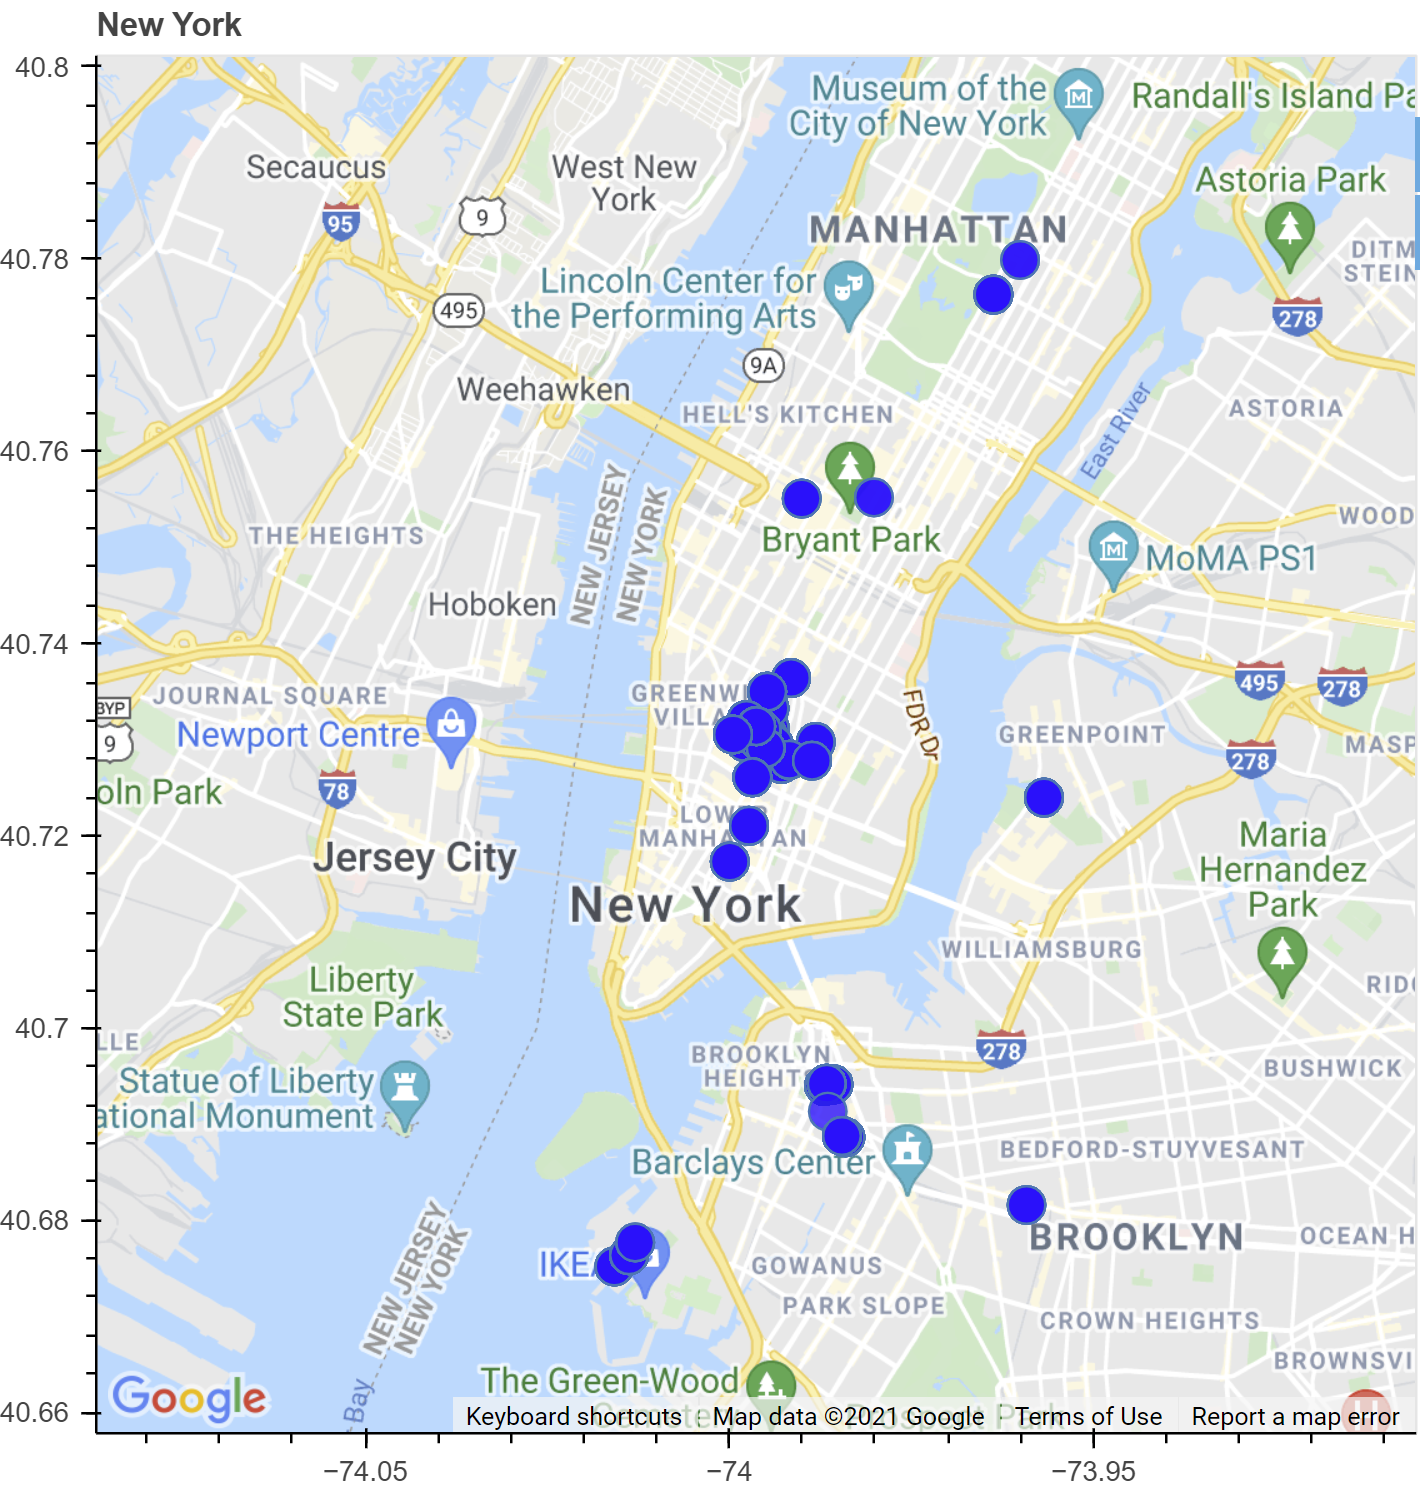
\includegraphics[width=6cm]{figure12}
		\caption{Sensors located on the map}
	\end{figure}

	Based on the figure (Fig. 7.), the ground truth is visualized against the predicted values of the data set from the sensors. We can observe that against the sounds in ground truth, the predictions are consistent. For instance, the sensors which detect the sound 6-1 stationary-music, the predicted sounds are mostly person-or-small-group-talking or car-horn or dog-barking. We can assume that people who play stationary music don't prefer to play in loud sounds like large-sounding-engine.  

	\begin{figure}[h!]
		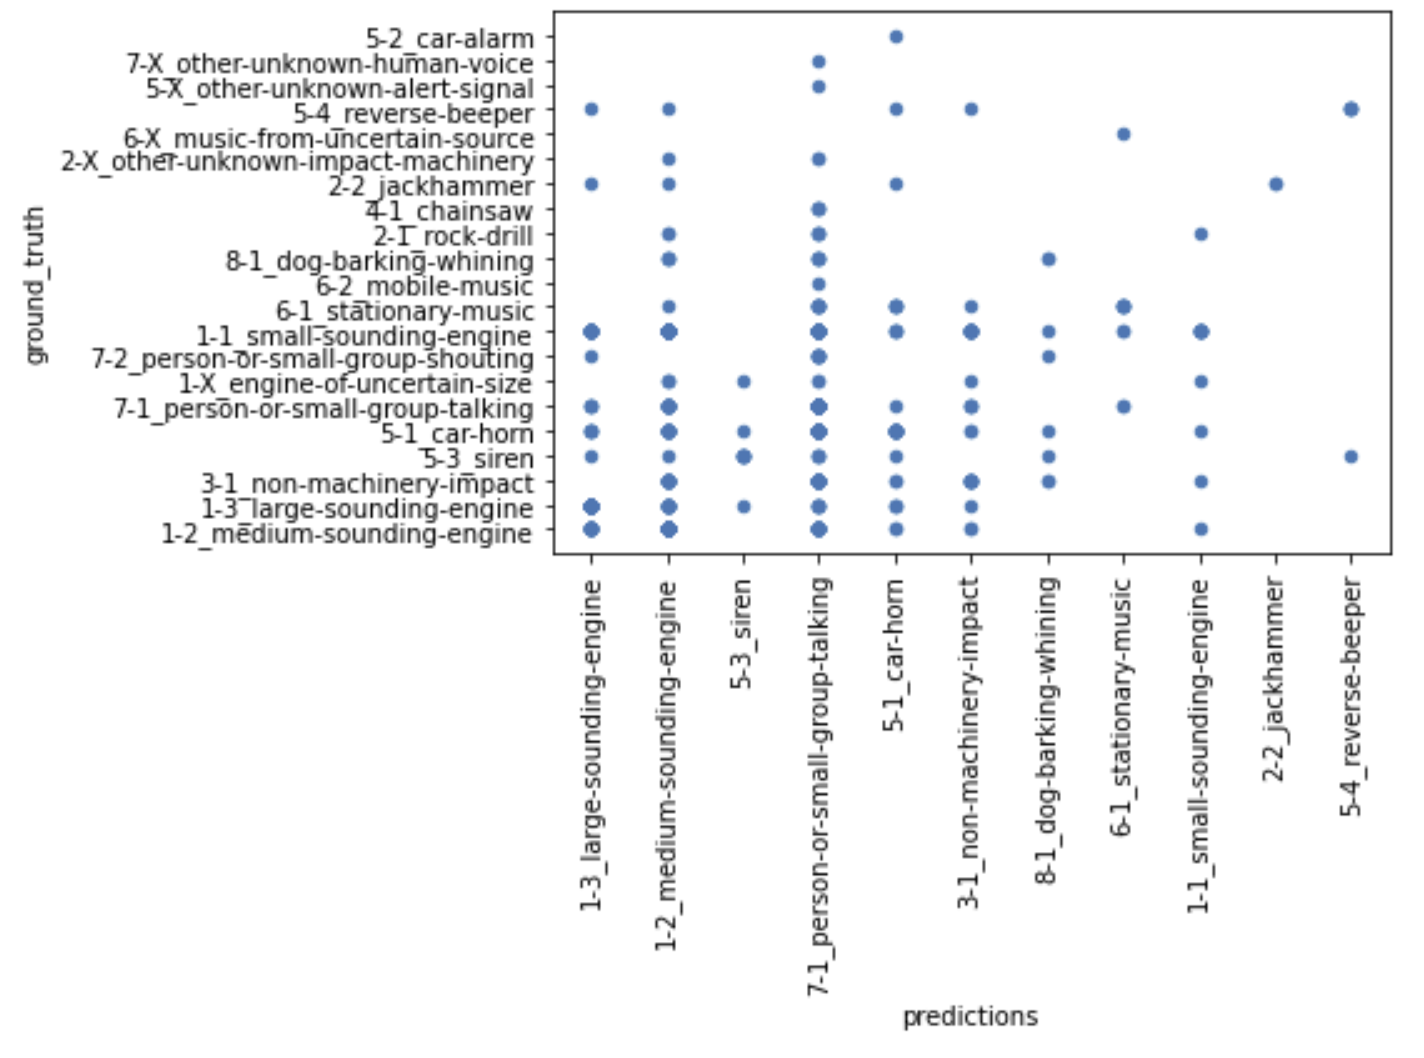
\includegraphics[width=9cm]{figure7}
		\caption{Predictions vs ground truth}
	\end{figure}

	The mismatches detected from the sensors tells us that there seem to be more occurring on Fridays, week days compared to weekends (Fig. 8.). Least number of mismatches occurs on Sundays, we can estimate that less people would be working compared to other days.
	Similarly, more number of mismatches occur in morning and night hours (Fig. 9.). which we could assume that there could be more people heading to and returning from work and less mismatches between 12 and 16 hours.


	\begin{figure}[h!]
		\centering
		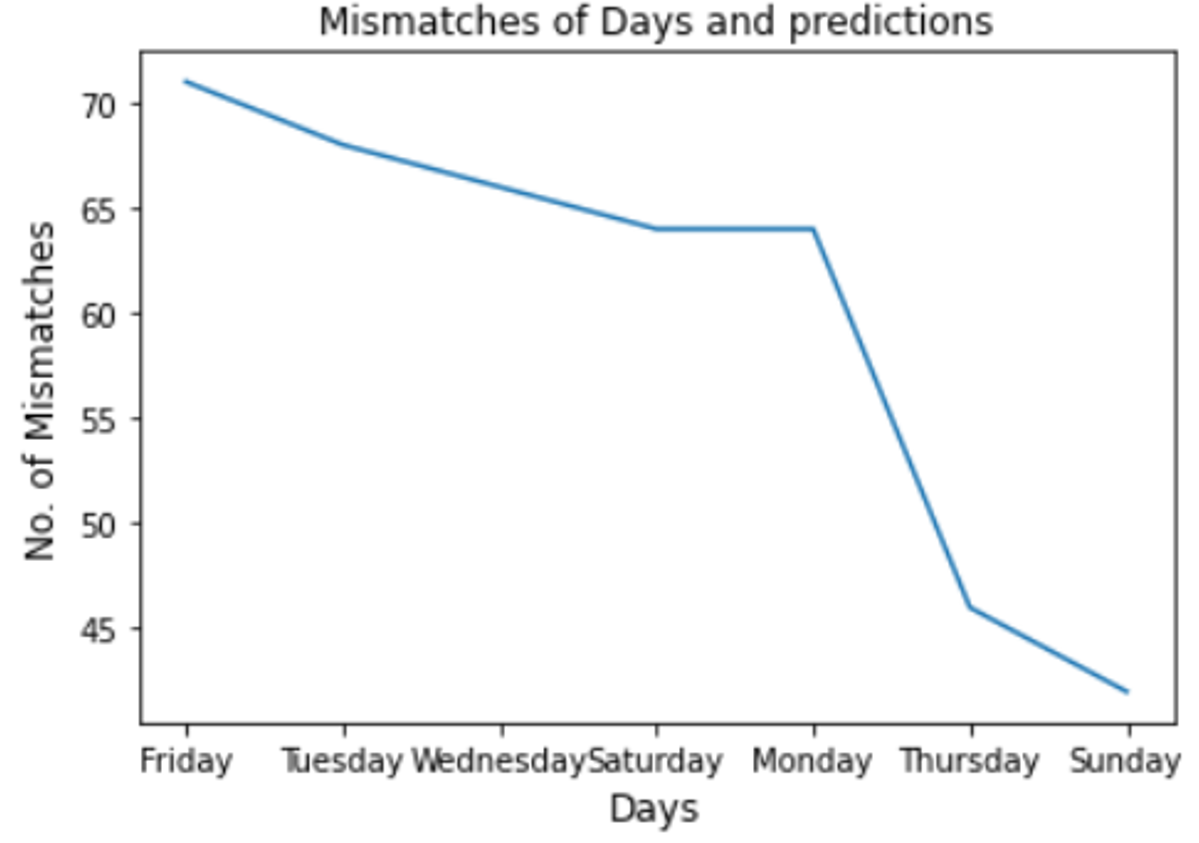
\includegraphics[width=4cm]{figure8}
		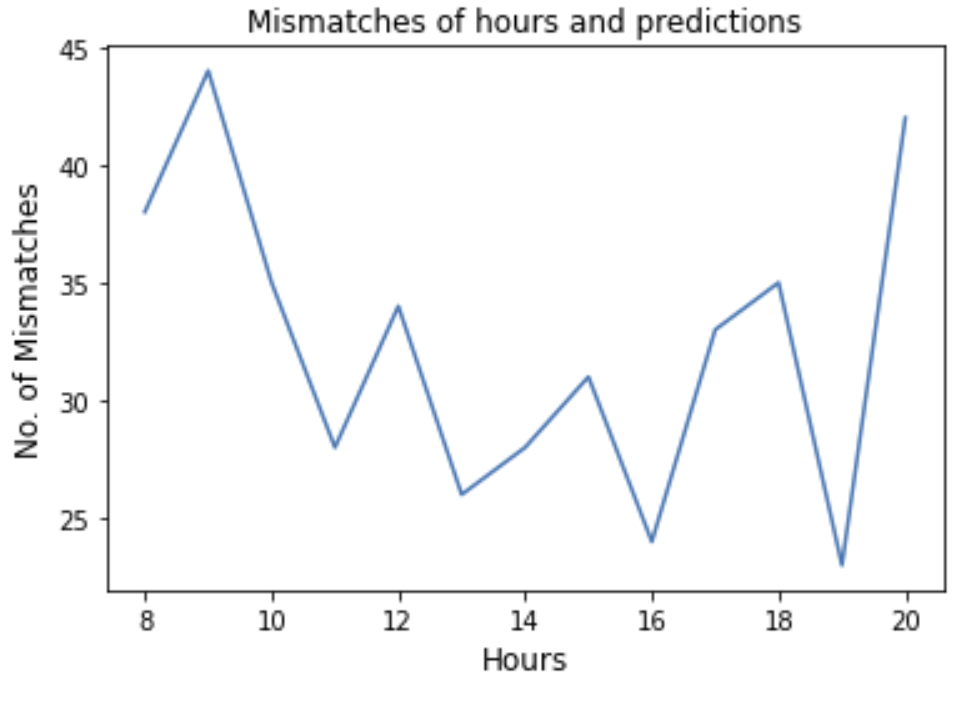
\includegraphics[width=4cm]{figure9}
		\caption{No. of mismatches vs Days, Hours}
	\end{figure}

	The different sensors located in and around the city recorded many sounds and after calculating the mismatches from them through ML model, we could see that most of the mismatches occur in 28th, the least in 53th sensor ((Fig. 10.). The reason could be that more number of mismatches could occur where there is more sounds being produced, where it is less accurate to identify each particular sound, where as the other sensor could be located around a zone where there are less sounds recorded.

	\begin{figure}[h!]
		\centering
		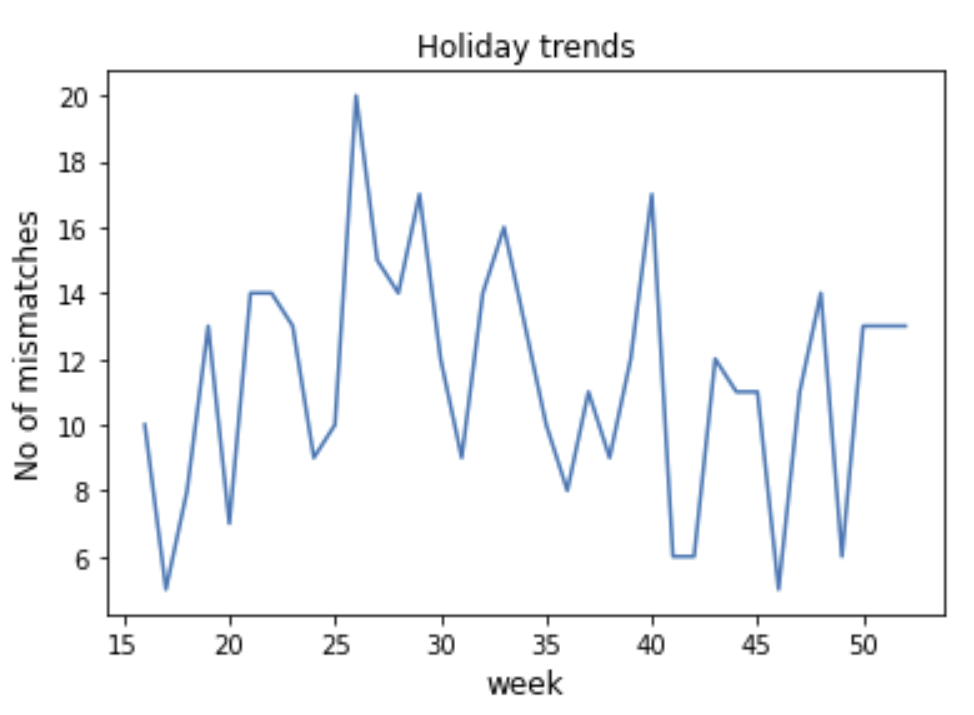
\includegraphics[width=7cm]{figure10}
		\caption{No. of mismatches vs Sensors}
	\end{figure}

	When we further analyzed the data for any trends generated in holidays, there was an interesting pattern visible from the mismatches (Fig. 11.). The week of July 4th (week 27) saw an increase in the number of mismatches compared to rest of the year in 2019 which could be as a result of holiday weekend, more sounds are detected by the sensors across Manhattan city compared to rest of the year, there was an increase in number of mismatches. We could identify holidays in the year through sudden increase in the number of mismatches as seen the below figure.

	\begin{figure}[h!]
		\centering
		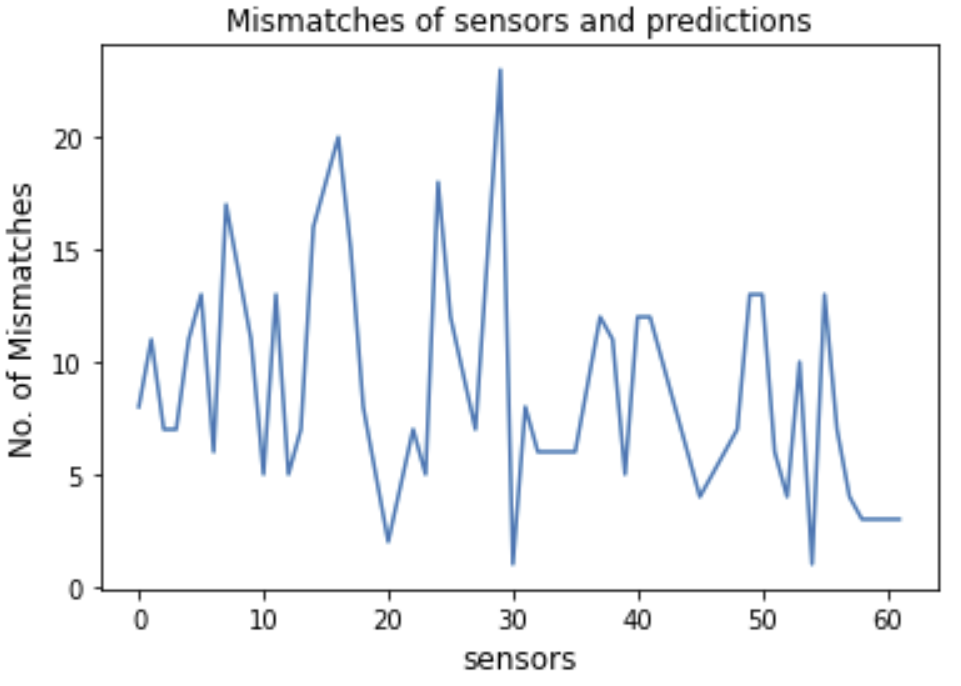
\includegraphics[width=7cm]{figure11}
		\caption{Holiday trends through mismatches}
	\end{figure}
